\documentclass{article}
\usepackage[utf8]{inputenc}
\usepackage{listings}

\title{Trabalho de Processamento de Imagem}
\author{Gustavo Diel & Marlon Henry Schweigert}
\date{Setembro de 2016}

\usepackage{natbib}
\usepackage{graphicx}

\usepackage{placeins}

\begin{document}

\maketitle

\section{Introdução}
Este documento refere-se ao resultado obtido do trabalho prático de Processamento de Imagem. 
Para este trabalho, implementamos diversas funções de processamento de imagem em Python. O principal objetivo desse trabalho é ressaltar o processamento e o resultado deste a fim de estudar as técnicas de:
Funções lineares
Funções não lineares
Equalização global
Equalização Local
Linearização

\newpage
\section{Transformações Lineares}

São funções que permitem aplicar a cada pixel uma função linear para alterar o contraste, dimenções, rotação, entre outros.

\lstinputlisting[language=Python]
{source001.py}

\begin{figure}[!htb]
\begin{minipage}[b]{0.45\linewidth}
\centering
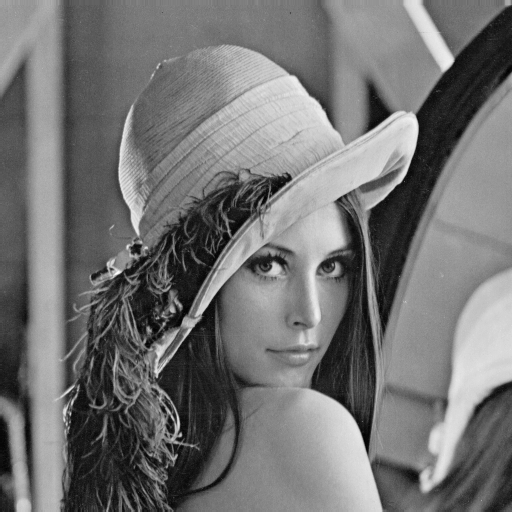
\includegraphics[scale=0.32]{lena_B.png}
\caption{Imagem Original}
\label{fig:original}
\end{minipage}
\hspace{0.5cm}
\begin{minipage}[b]{0.45\linewidth}
\centering
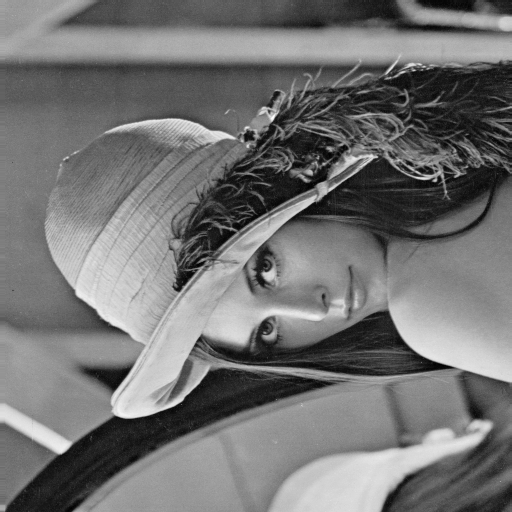
\includegraphics[scale=0.32]{TransLinearRot.png}
\caption{Imagem Rotacionada}
\label{fig:rota}
\end{minipage}
\end{figure}
\FloatBarrier
\begin{figure}[!htb]
\begin{minipage}[b]{0.45\linewidth}
\centering
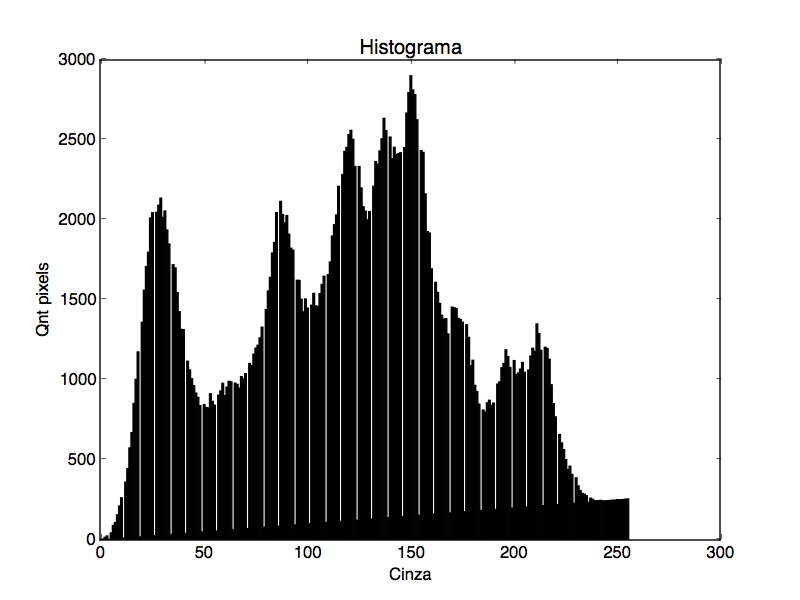
\includegraphics[scale=0.25]{Histo_lena_B.jpg}
\caption{Imagem Original}
\label{fig:original}
\end{minipage}
\hspace{0.5cm}
\begin{minipage}[b]{0.45\linewidth}
\centering
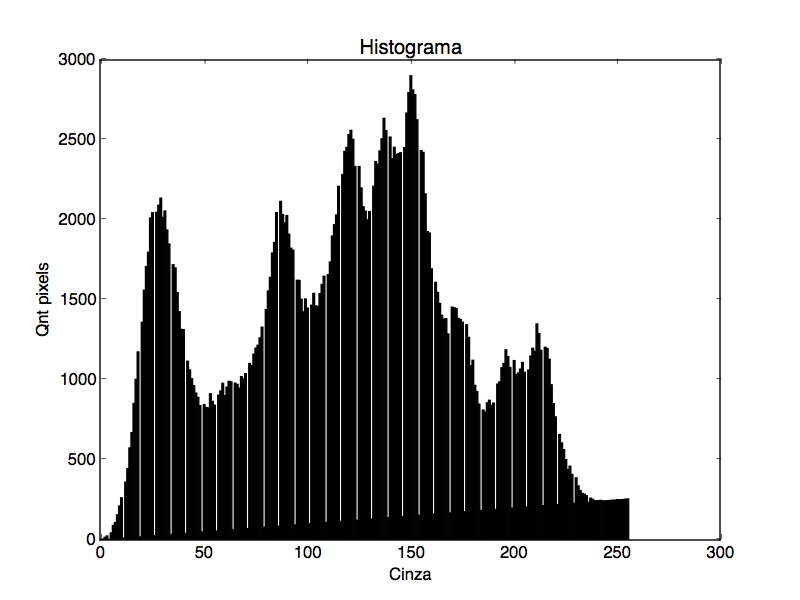
\includegraphics[scale=0.25]{Histo_TransLinearRot.jpg}
\caption{Imagem Rotacionada}
\label{fig:rota}
\end{minipage}
\end{figure}
\FloatBarrier

\newpage

Neste exemplo, aplicamos uma função linar não centrada $f(x) = (2*x + 47) / 2$ em toda a imagem.

Por ser um coeficiente de deslocamento baixo, houve pouca alteração.


\begin{figure}[!htb]
\begin{minipage}[b]{0.45\linewidth}
\centering
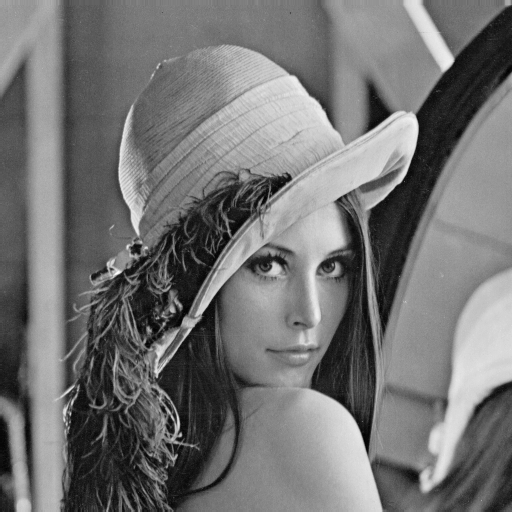
\includegraphics[scale=0.32]{lena_B.png}
\caption{Imagem Original}
\label{fig:original}
\end{minipage}
\hspace{0.5cm}
\begin{minipage}[b]{0.45\linewidth}
\centering
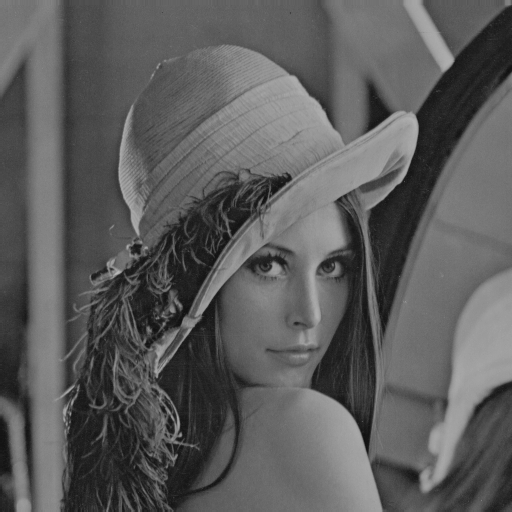
\includegraphics[scale=0.32]{TransLinearSimples.png}
\caption{Transformação linear}
\label{fig:rota}
\end{minipage}
\end{figure}
\FloatBarrier
\begin{figure}[!htb]
\begin{minipage}[b]{0.45\linewidth}
\centering
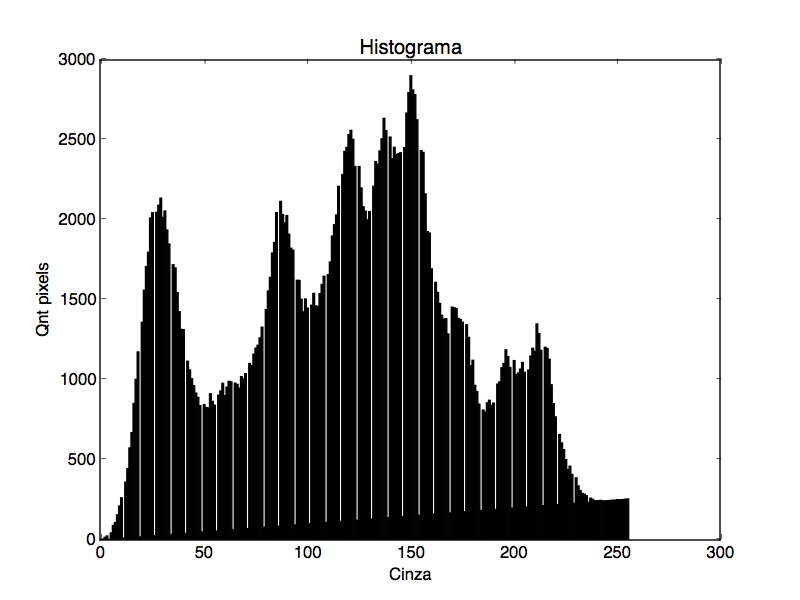
\includegraphics[scale=0.25]{Histo_lena_B.jpg}
\caption{Imagem Original}
\label{fig:original}
\end{minipage}
\hspace{0.5cm}
\begin{minipage}[b]{0.45\linewidth}
\centering
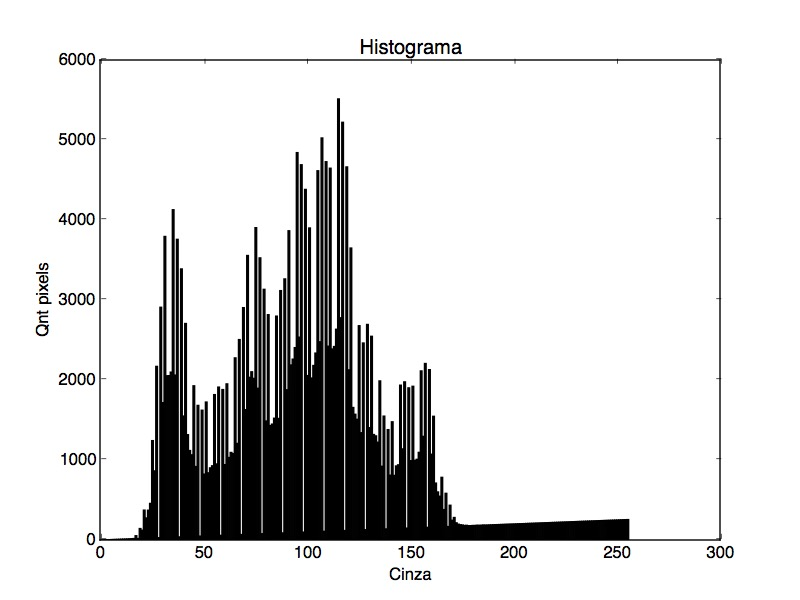
\includegraphics[scale=0.25]{Histo_TransLinearSimples.jpg}
\caption{Transformação Linear}
\label{fig:rota}
\end{minipage}
\end{figure}
\FloatBarrier

\newpage
\section{Transformações Não Linear}

São funções que permitem aplicar a cada pixel uma função não linear para alterar suas propriedades.
\lstinputlisting[language=Python]
{source002.py}

\newpage

\begin{figure}[!htb]
\begin{minipage}[b]{0.45\linewidth}
\centering
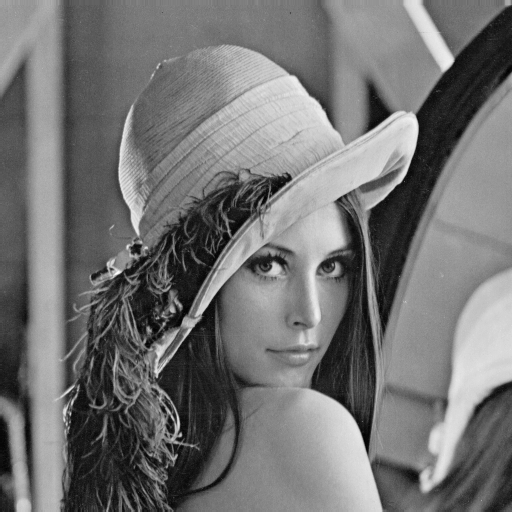
\includegraphics[scale=0.32]{lena_B.png}
\caption{Imagem Original}
\label{fig:original}
\end{minipage}
\hspace{0.5cm}
\begin{minipage}[b]{0.45\linewidth}
\centering
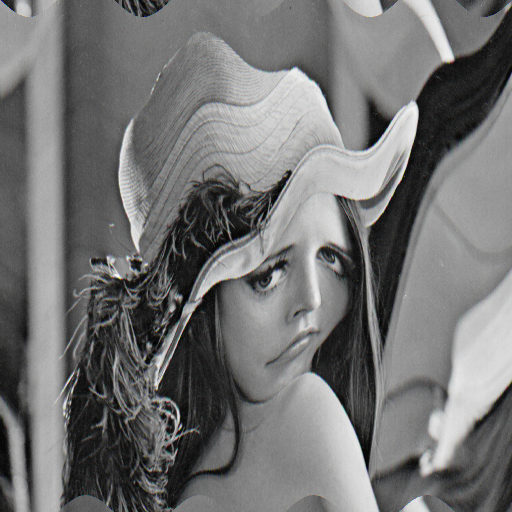
\includegraphics[scale=0.32]{TransNaoLinearDistorcao.png}
\caption{Imagem Rotacionada}
\label{fig:rota}
\end{minipage}
\end{figure}
\FloatBarrier
\begin{figure}[!htb]
\begin{minipage}[b]{0.45\linewidth}
\centering
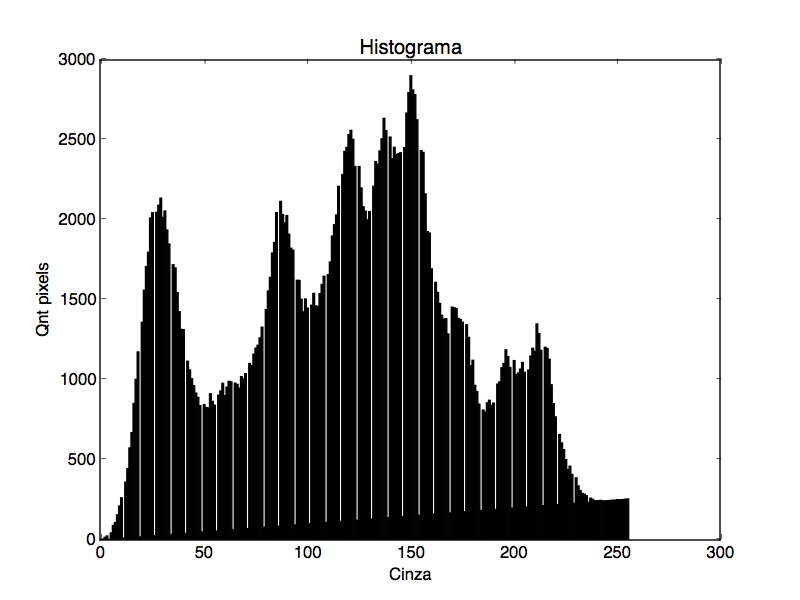
\includegraphics[scale=0.25]{Histo_lena_B.jpg}
\caption{Imagem Original}
\label{fig:original}
\end{minipage}
\hspace{0.5cm}
\begin{minipage}[b]{0.45\linewidth}
\centering
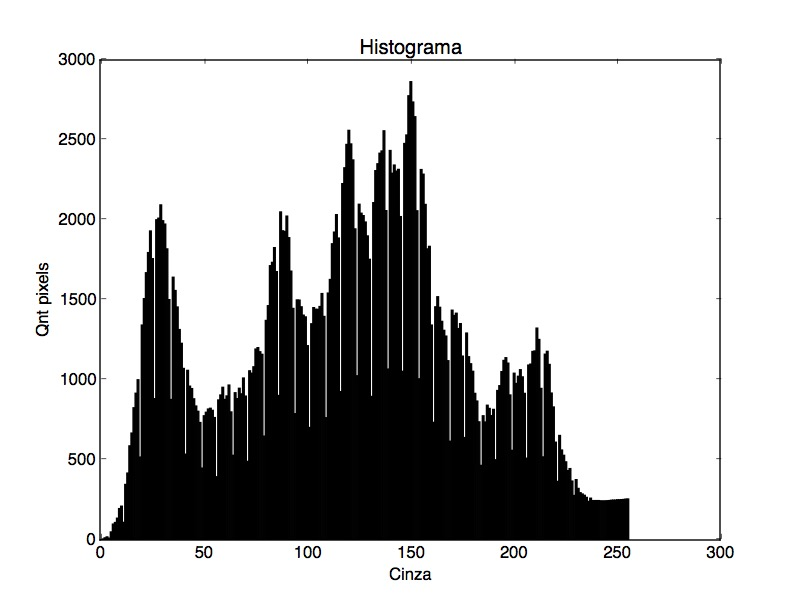
\includegraphics[scale=0.25]{Histo_TransNaoLinearDistorcao.jpg}
\caption{Imagem Rotacionada}
\label{fig:rota}
\end{minipage}
\end{figure}
\FloatBarrier

\newpage
\begin{figure}[!htb]
\begin{minipage}[b]{0.45\linewidth}
\centering
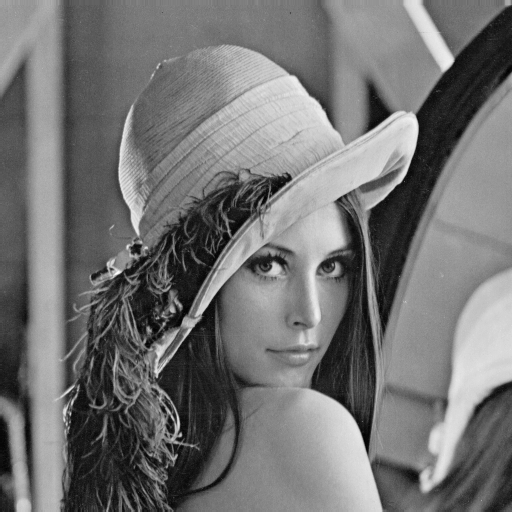
\includegraphics[scale=0.32]{lena_B.png}
\caption{Imagem Original}
\label{fig:original}
\end{minipage}
\hspace{0.5cm}
\begin{minipage}[b]{0.45\linewidth}
\centering
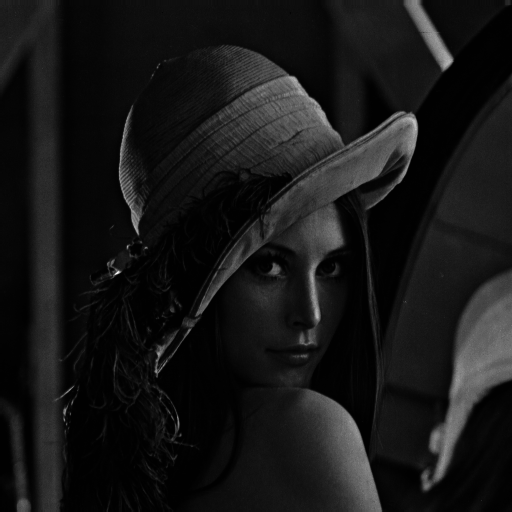
\includegraphics[scale=0.32]{TransNLinearExp.png}
\caption{Função Exponencial}
\label{fig:rota}
\end{minipage}
\end{figure}
\FloatBarrier
\begin{figure}[!htb]
\begin{minipage}[b]{0.45\linewidth}
\centering
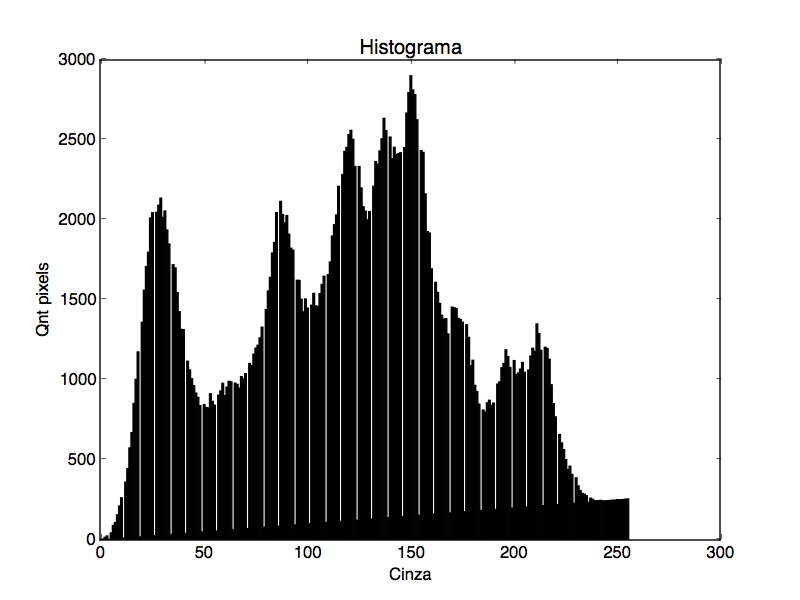
\includegraphics[scale=0.25]{Histo_lena_B.jpg}
\caption{Imagem Original}
\label{fig:original}
\end{minipage}
\hspace{0.5cm}
\begin{minipage}[b]{0.45\linewidth}
\centering
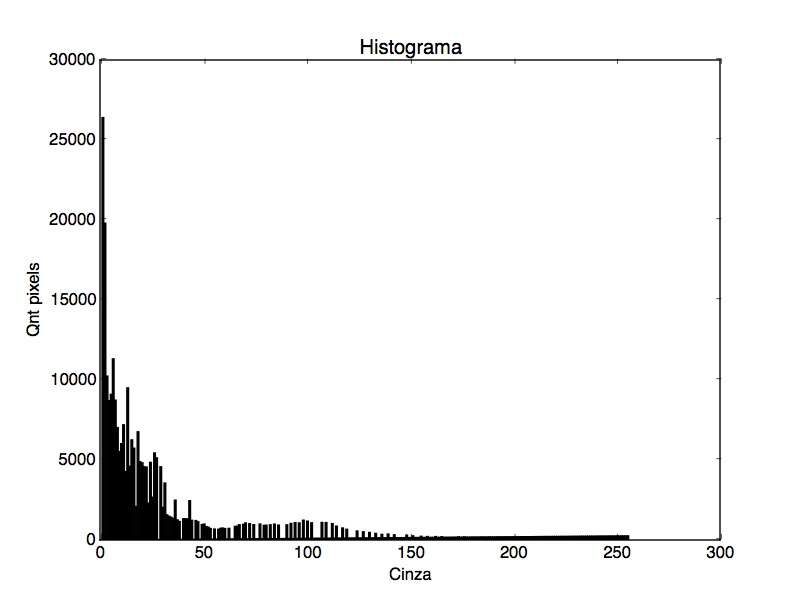
\includegraphics[scale=0.25]{Histo_TransNLinearExp.jpg}
\caption{Função Exponencial}
\label{fig:rota}
\end{minipage}
\end{figure}
\FloatBarrier

\newpage
\begin{figure}[!htb]
\begin{minipage}[b]{0.45\linewidth}
\centering
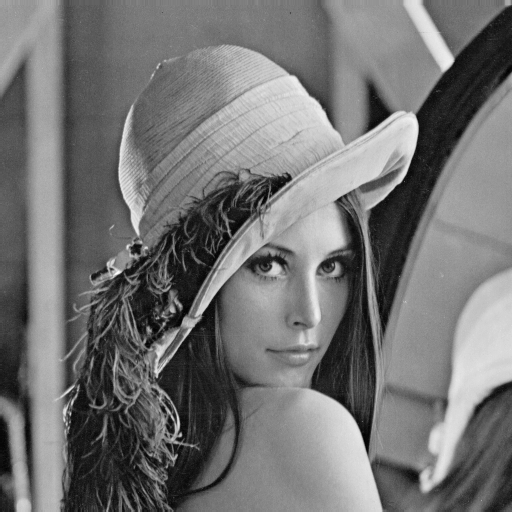
\includegraphics[scale=0.32]{lena_B.png}
\caption{Imagem Original}
\label{fig:original}
\end{minipage}
\hspace{0.5cm}
\begin{minipage}[b]{0.45\linewidth}
\centering
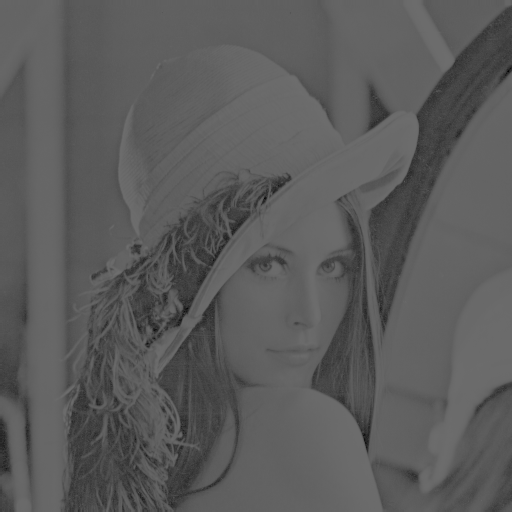
\includegraphics[scale=0.32]{TransNLinearLog.png}
\caption{Função Logarítmica}
\label{fig:rota}
\end{minipage}
\end{figure}
\FloatBarrier
\begin{figure}[!htb]
\begin{minipage}[b]{0.45\linewidth}
\centering
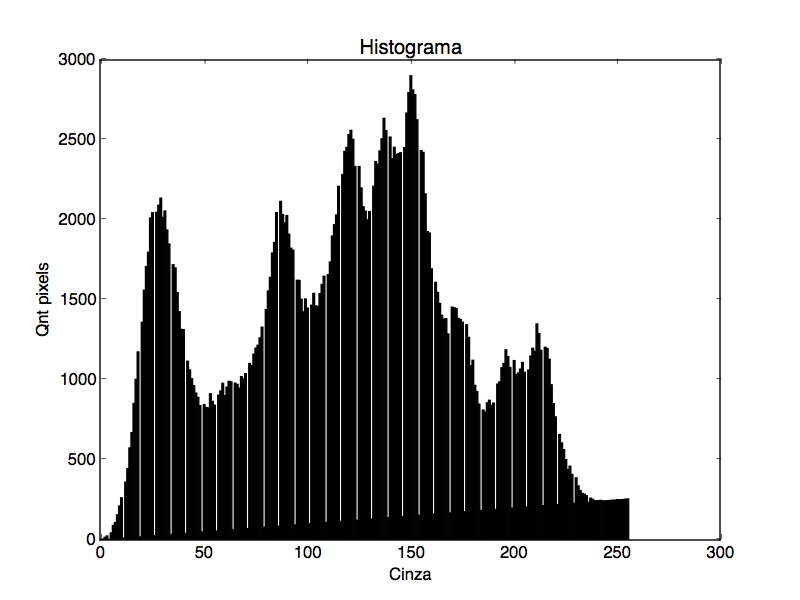
\includegraphics[scale=0.25]{Histo_lena_B.jpg}
\caption{Imagem Original}
\label{fig:original}
\end{minipage}
\hspace{0.5cm}
\begin{minipage}[b]{0.45\linewidth}
\centering
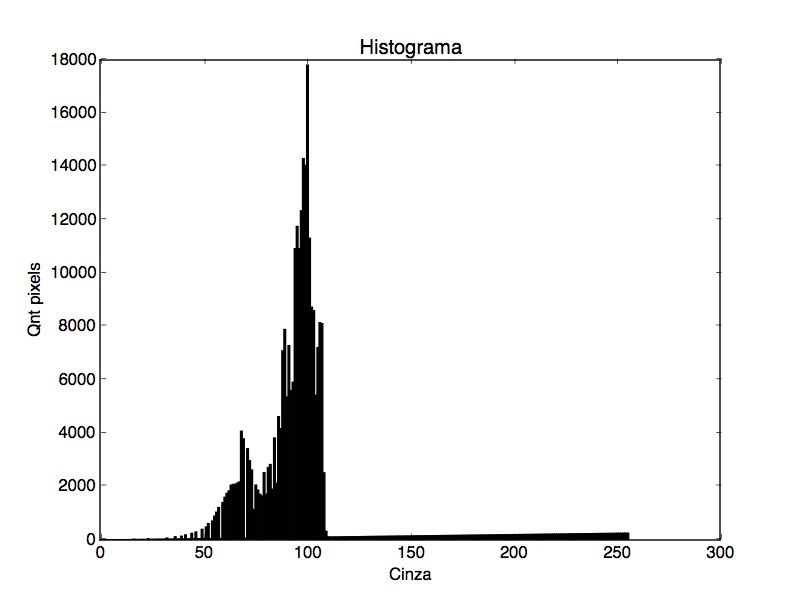
\includegraphics[scale=0.25]{Histo_TransNLinearLog.jpg}
\caption{Função Logarítmica}
\label{fig:rota}
\end{minipage}
\end{figure}
\FloatBarrier

\newpage
\begin{figure}[!htb]
\begin{minipage}[b]{0.45\linewidth}
\centering
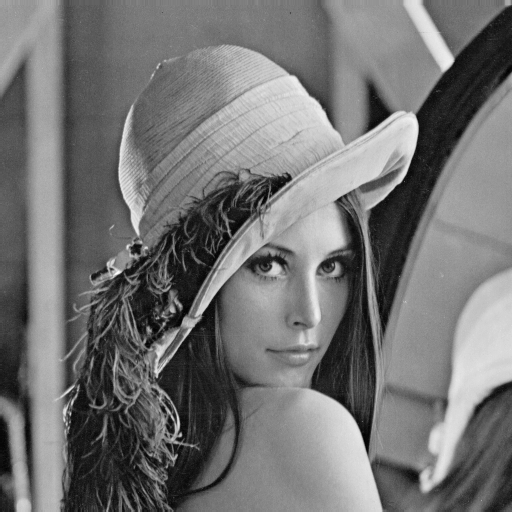
\includegraphics[scale=0.32]{lena_B.png}
\caption{Imagem Original}
\label{fig:original}
\end{minipage}
\hspace{0.5cm}
\begin{minipage}[b]{0.45\linewidth}
\centering

\includegraphics[scale=0.32]{TransNLinearRoot.png}
\caption{Função Raiz}
\label{fig:rota}
\end{minipage}
\end{figure}
\FloatBarrier
\begin{figure}[!htb]
\begin{minipage}[b]{0.45\linewidth}
\centering
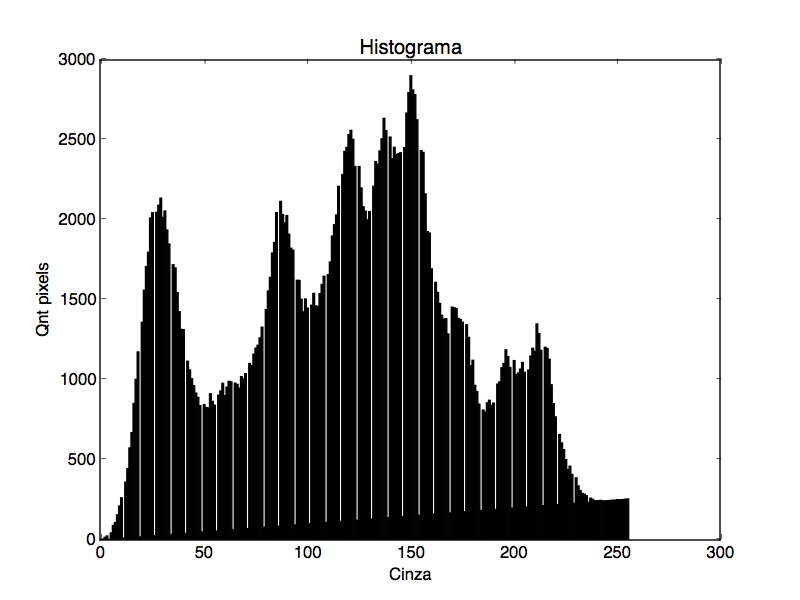
\includegraphics[scale=0.25]{Histo_lena_B.jpg}
\caption{Imagem Original}
\label{fig:original}
\end{minipage}
\hspace{0.5cm}
\begin{minipage}[b]{0.45\linewidth}
\centering
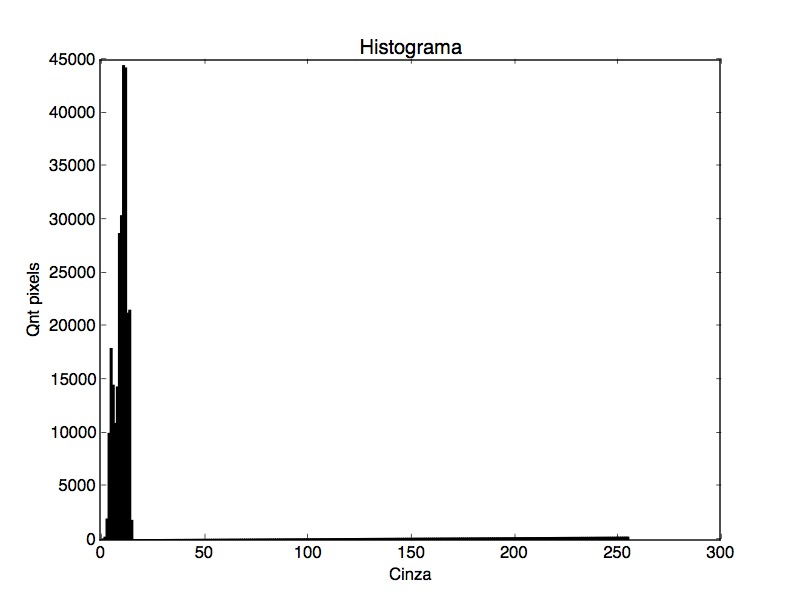
\includegraphics[scale=0.25]{Histo_TransNLinearRoot.jpg}
\caption{Função Raiz}
\label{fig:rota}
\end{minipage}
\end{figure}
\FloatBarrier

\newpage
\begin{figure}[!htb]
\begin{minipage}[b]{0.45\linewidth}
\centering
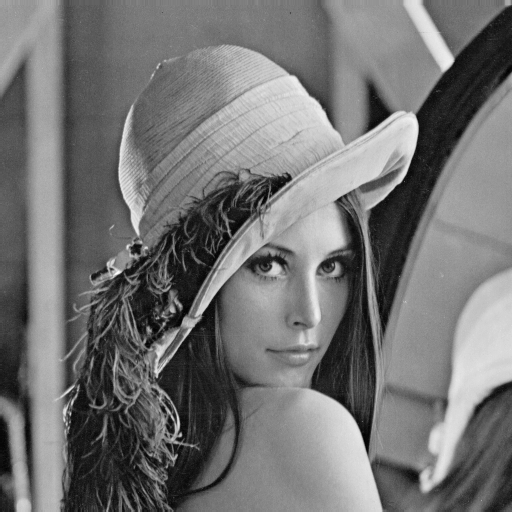
\includegraphics[scale=0.32]{lena_B.png}
\caption{Imagem Original}
\label{fig:original}
\end{minipage}
\hspace{0.5cm}
\begin{minipage}[b]{0.45\linewidth}
\centering
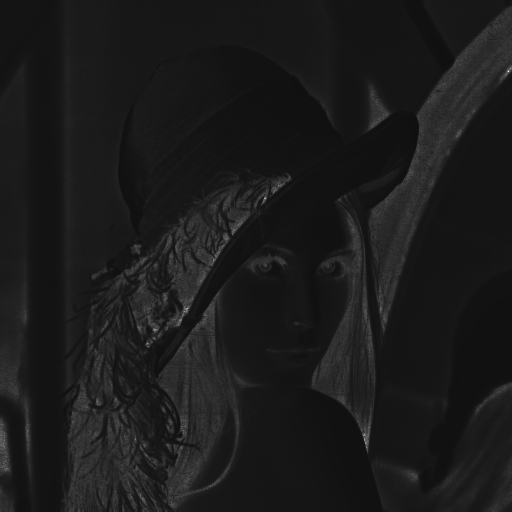
\includegraphics[scale=0.32]{TransNLinearRootInv.png}
\caption{Função Raiz Inversa}
\label{fig:rota}
\end{minipage}
\end{figure}
\FloatBarrier
\begin{figure}[!htb]
\begin{minipage}[b]{0.45\linewidth}
\centering
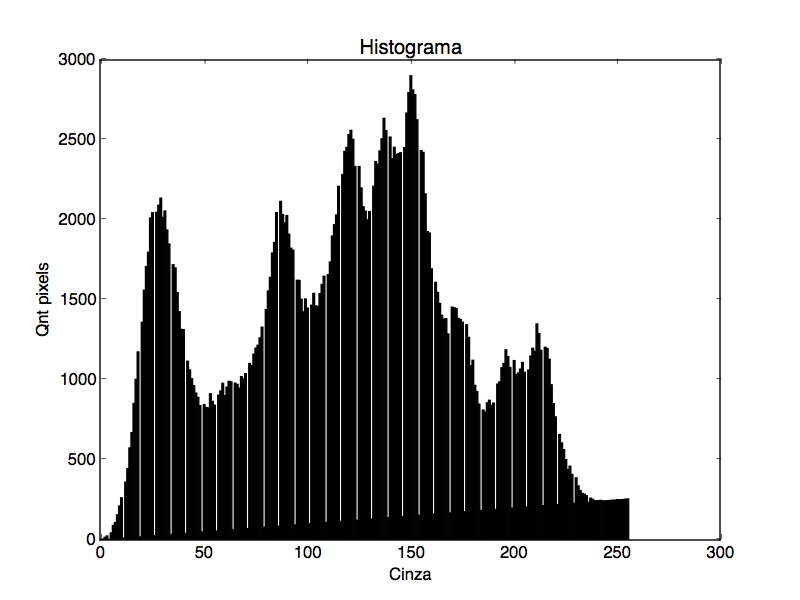
\includegraphics[scale=0.25]{Histo_lena_B.jpg}
\caption{Imagem Original}
\label{fig:original}
\end{minipage}
\hspace{0.5cm}
\begin{minipage}[b]{0.45\linewidth}
\centering
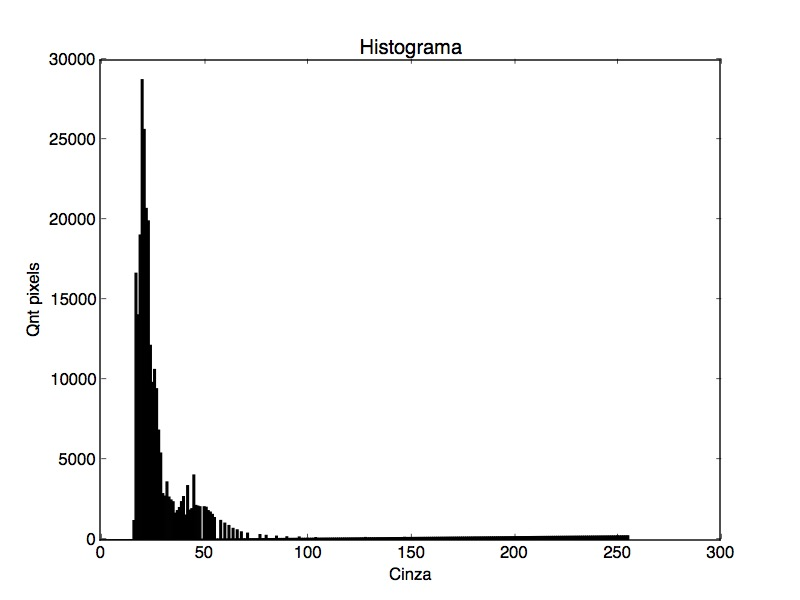
\includegraphics[scale=0.25]{Histo_TransNLinearRootInv.jpg}
\caption{Funcão Raiz Inversa}
\label{fig:rota}
\end{minipage}
\end{figure}
\FloatBarrier

\newpage
\section{Equalização}
Aplicação das funcoes de equalizacao estudadas em sala.
\lstinputlisting[language=Python]
{Trab_HistGlobal.py}

\newpage

\begin{figure}[!htb]
\begin{minipage}[b]{0.45\linewidth}
\centering
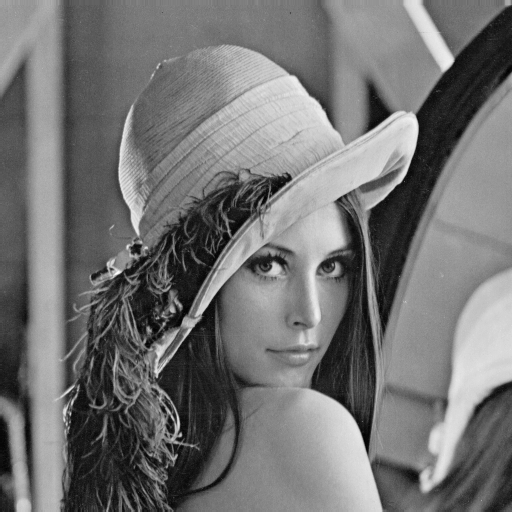
\includegraphics[scale=0.32]{lena_B.png}
\caption{Imagem Original}
\label{fig:original}
\end{minipage}
\hspace{0.5cm}
\begin{minipage}[b]{0.45\linewidth}
\centering
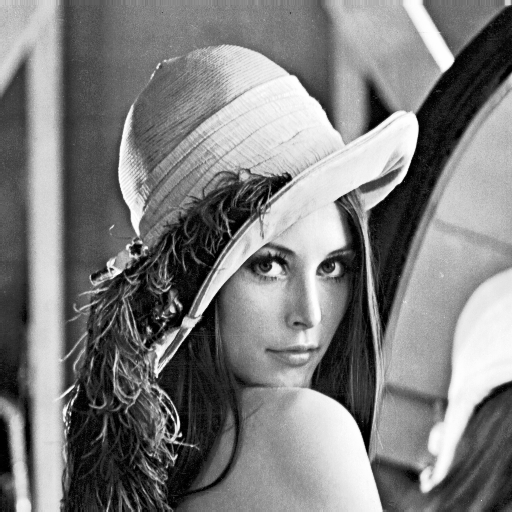
\includegraphics[scale=0.32]{EqGlobal.png}
\caption{Equalização Global}
\label{fig:rota}
\end{minipage}
\end{figure}
\FloatBarrier
\begin{figure}[!htb]
\begin{minipage}[b]{0.45\linewidth}
\centering
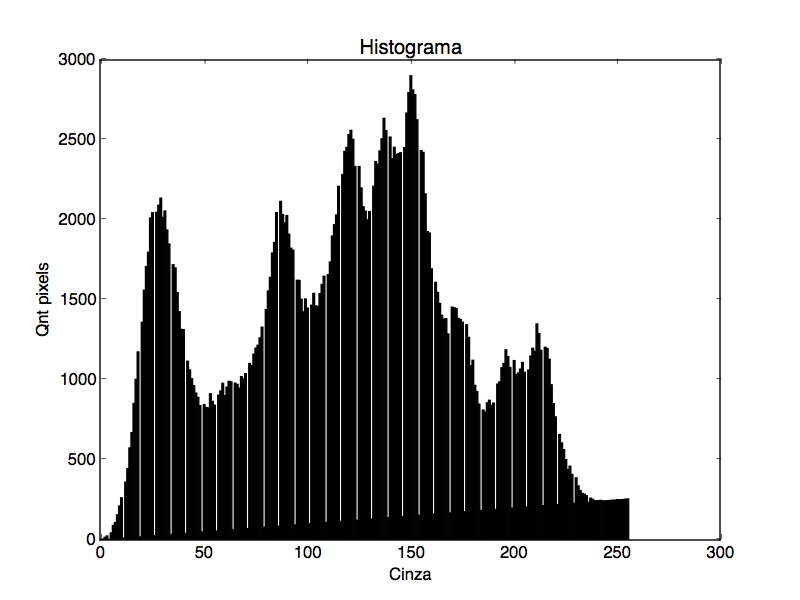
\includegraphics[scale=0.25]{Histo_lena_B.jpg}
\caption{Imagem Original}
\label{fig:original}
\end{minipage}
\hspace{0.5cm}
\begin{minipage}[b]{0.45\linewidth}
\centering
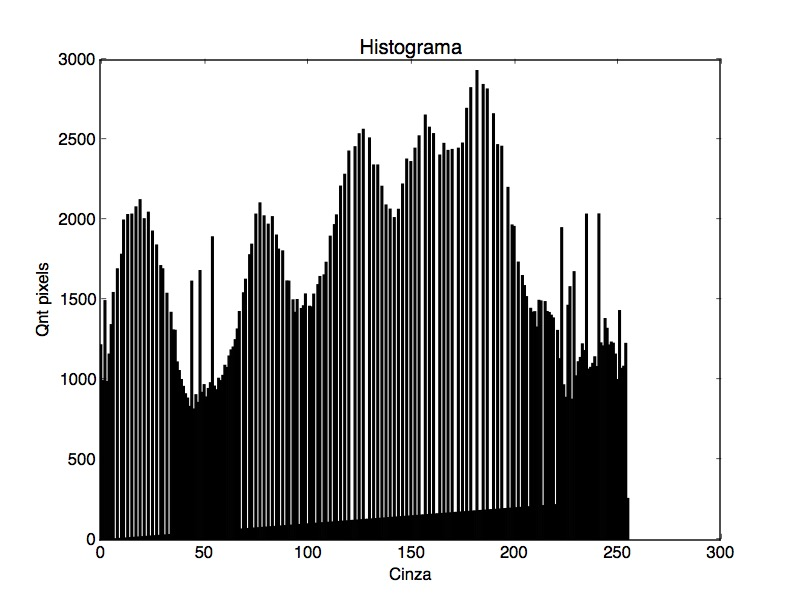
\includegraphics[scale=0.25]{Histo_EqGlobal.jpg}
\caption{Equalização Global}
\label{fig:rota}
\end{minipage}
\end{figure}
\FloatBarrier

\newpage
\begin{figure}[!htb]
\begin{minipage}[b]{0.45\linewidth}
\centering
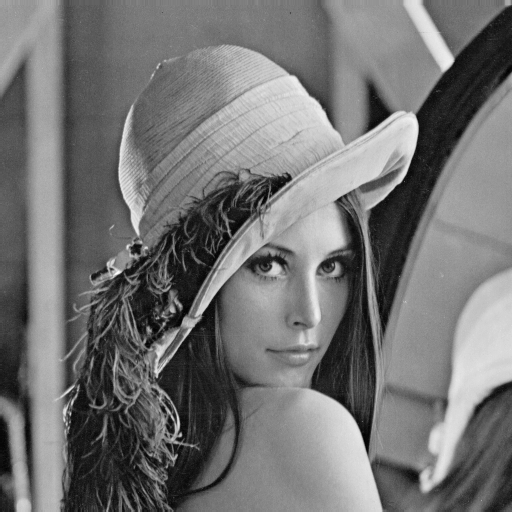
\includegraphics[scale=0.32]{lena_B.png}
\caption{Imagem Original}
\label{fig:original}
\end{minipage}
\hspace{0.5cm}
\begin{minipage}[b]{0.45\linewidth}
\centering
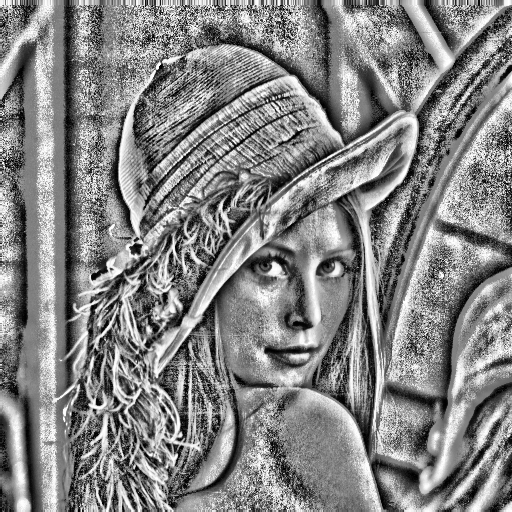
\includegraphics[scale=0.32]{EqLocal.png}
\caption{Equalizacao Local}
\label{fig:rota}
\end{minipage}
\end{figure}
\FloatBarrier
\begin{figure}[!htb]
\begin{minipage}[b]{0.45\linewidth}
\centering
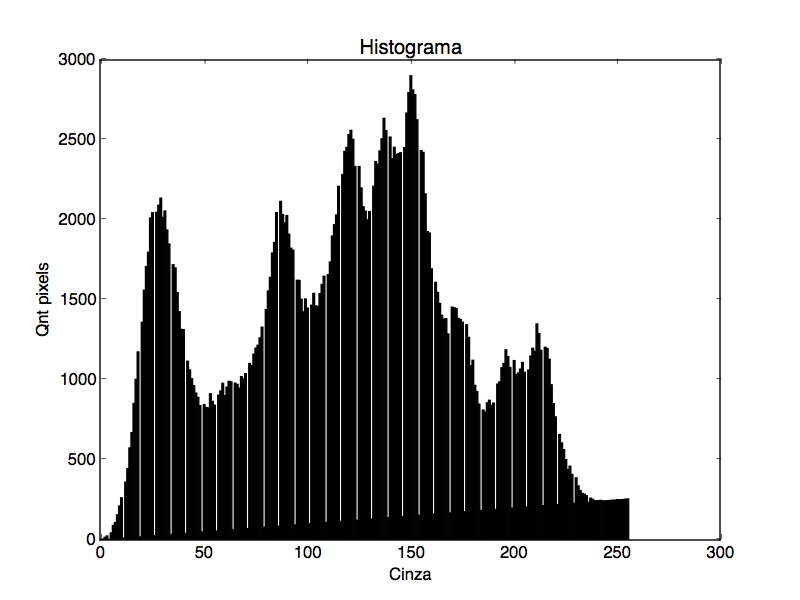
\includegraphics[scale=0.25]{Histo_lena_B.jpg}
\caption{Imagem Original}
\label{fig:original}
\end{minipage}
\hspace{0.5cm}
\begin{minipage}[b]{0.45\linewidth}
\centering
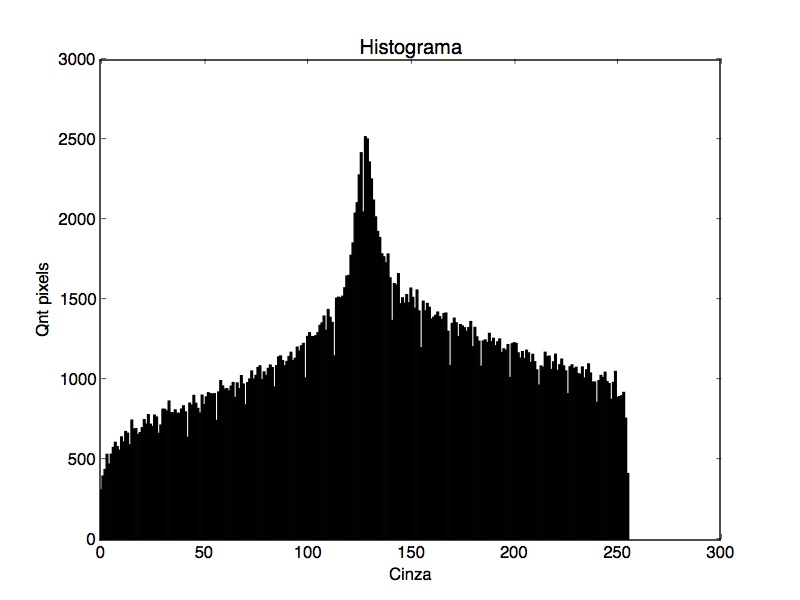
\includegraphics[scale=0.25]{Histo_EqLocal.jpg}
\caption{Equalizacao Local}
\label{fig:rota}
\end{minipage}
\end{figure}
\FloatBarrier

\newpage
\section{Linearização}
Nestes tres exemplos a seguir, iremos linearizar a imagem de 3 modos. Um simples, outro em 3 escalas de cinza e o ultimo com um número n de escalas.
\lstinputlisting[language=Python]
{Trab_DiminuirBits.py}

\newpage

\begin{figure}[!htb]
\begin{minipage}[b]{0.45\linewidth}
\centering
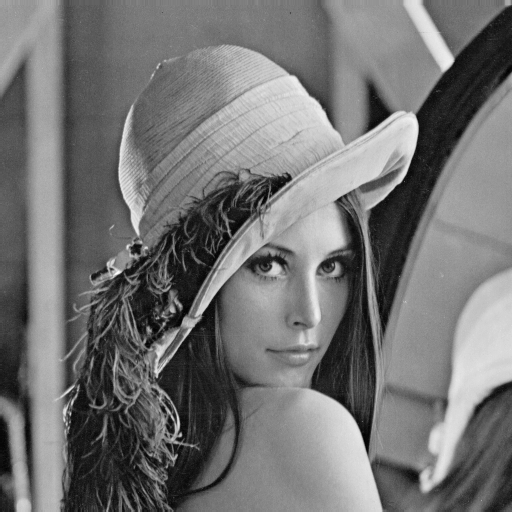
\includegraphics[scale=0.32]{lena_B.png}
\caption{Imagem Original}
\label{fig:original}
\end{minipage}
\hspace{0.5cm}
\begin{minipage}[b]{0.45\linewidth}
\centering
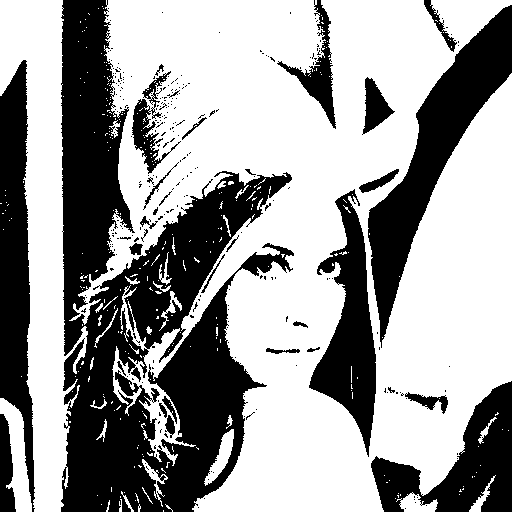
\includegraphics[scale=0.32]{Linearizacao.png}
\caption{Linearização Simples}
\label{fig:rota}
\end{minipage}
\end{figure}
\FloatBarrier
\begin{figure}[!htb]
\begin{minipage}[b]{0.45\linewidth}
\centering
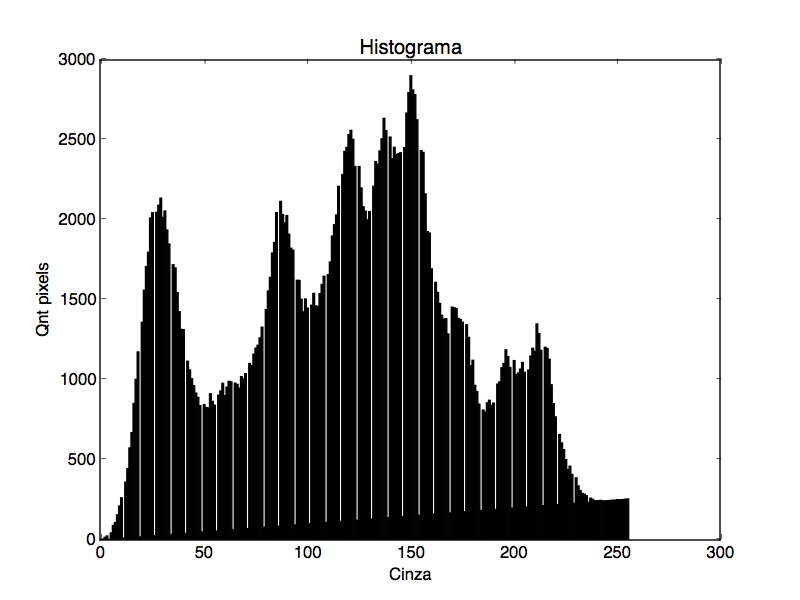
\includegraphics[scale=0.25]{Histo_lena_B.jpg}
\caption{Imagem Original}
\label{fig:original}
\end{minipage}
\hspace{0.5cm}
\begin{minipage}[b]{0.45\linewidth}
\centering
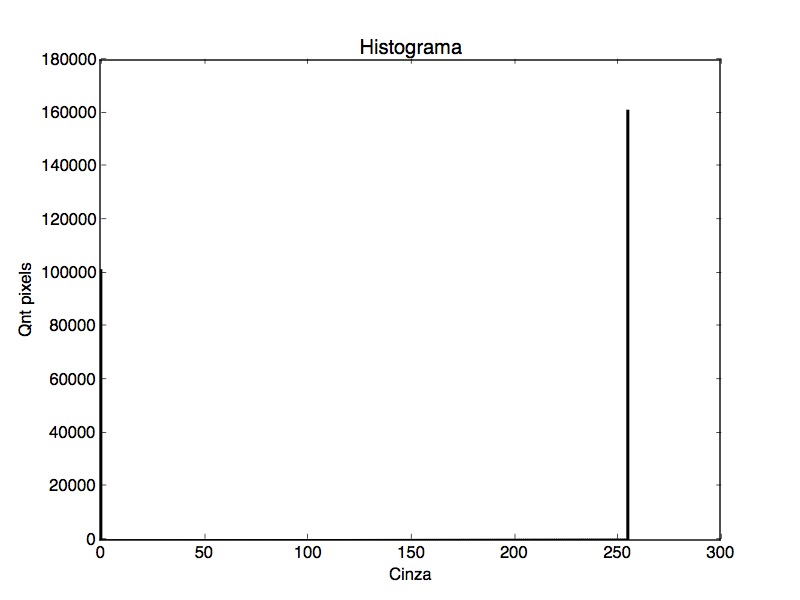
\includegraphics[scale=0.25]{Histo_Linearizacao.jpg}
\caption{Linearização Simples}
\label{fig:rota}
\end{minipage}
\end{figure}
\FloatBarrier

\newpage
\begin{figure}[!htb]
\begin{minipage}[b]{0.45\linewidth}
\centering
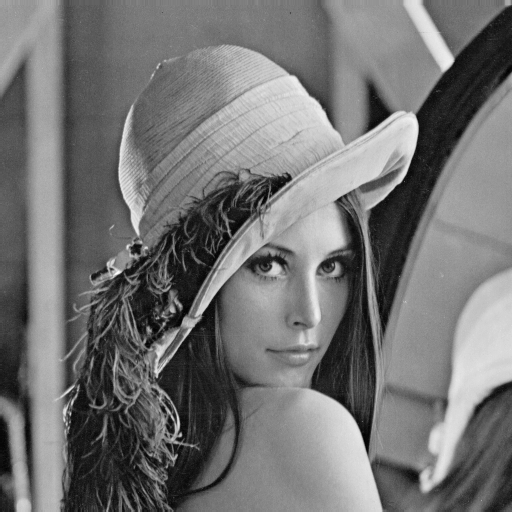
\includegraphics[scale=0.32]{lena_B.png}
\caption{Imagem Original}
\label{fig:original}
\end{minipage}
\hspace{0.5cm}
\begin{minipage}[b]{0.45\linewidth}
\centering
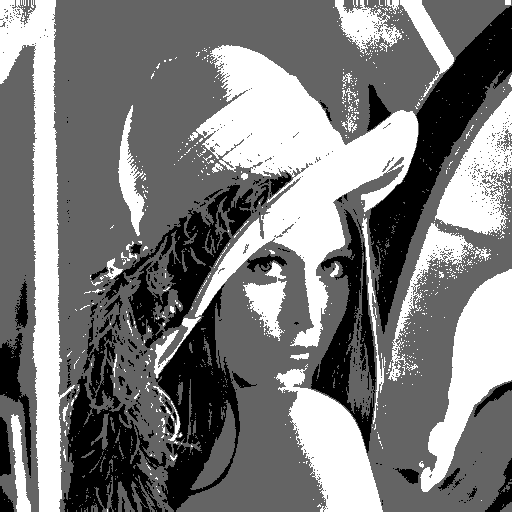
\includegraphics[scale=0.32]{LinearizacaoMultipla.png}
\caption{Linearização em 3 etapas}
\label{fig:rota}
\end{minipage}
\end{figure}
\FloatBarrier
\begin{figure}[!htb]
\begin{minipage}[b]{0.45\linewidth}
\centering
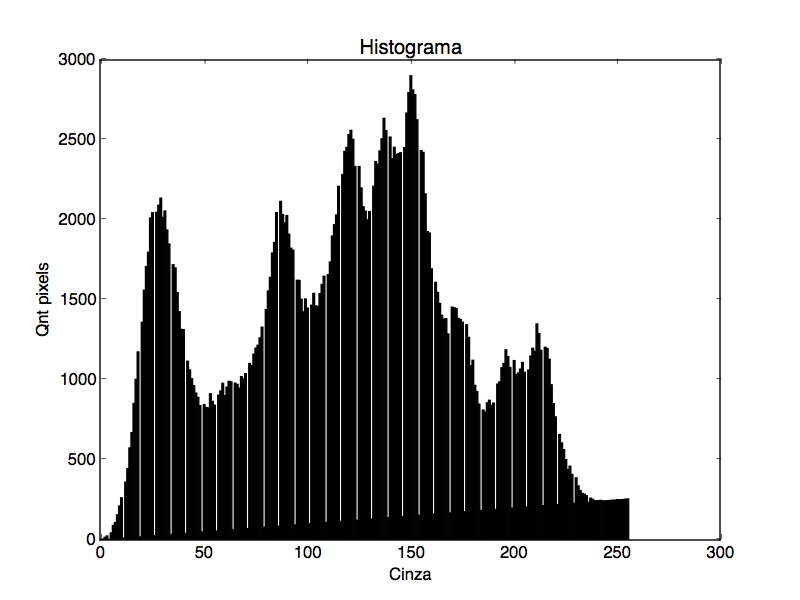
\includegraphics[scale=0.25]{Histo_lena_B.jpg}
\caption{Imagem Original}
\label{fig:original}
\end{minipage}
\hspace{0.5cm}
\begin{minipage}[b]{0.45\linewidth}
\centering
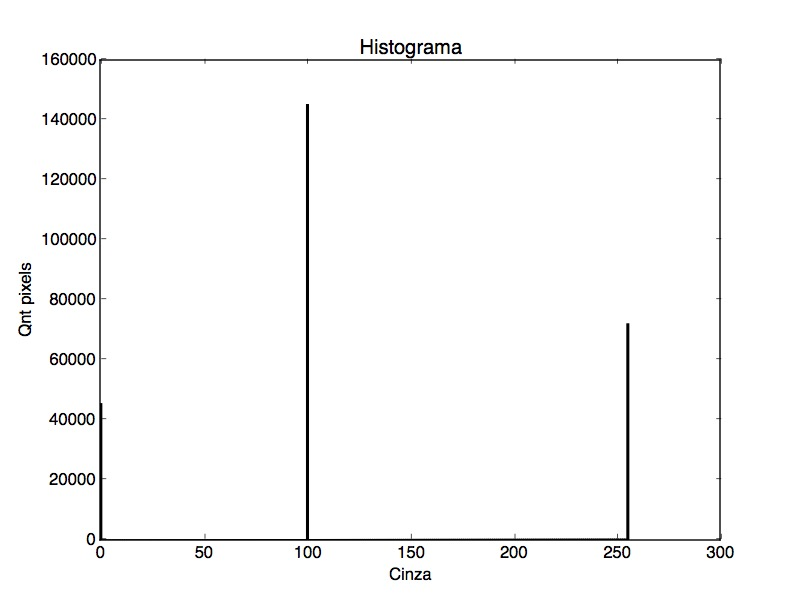
\includegraphics[scale=0.25]{Histo_LinearizacaoMultipla.jpg}
\caption{Linearização em 3 etapas}
\label{fig:rota}
\end{minipage}
\end{figure}
\FloatBarrier

\newpage
\begin{figure}[!htb]
\begin{minipage}[b]{0.45\linewidth}
\centering
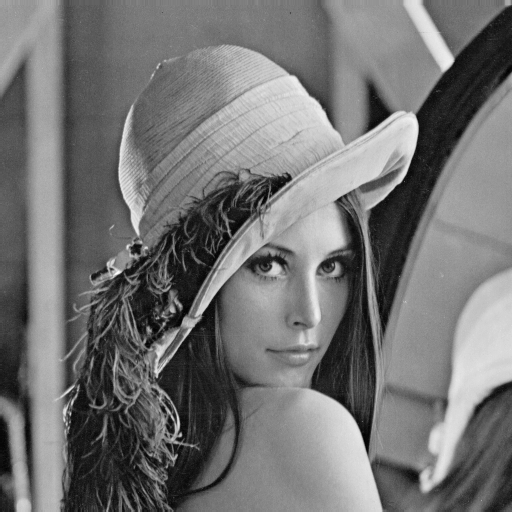
\includegraphics[scale=0.32]{lena_B.png}
\caption{Imagem Original}
\label{fig:original}
\end{minipage}
\hspace{0.5cm}
\begin{minipage}[b]{0.45\linewidth}
\centering
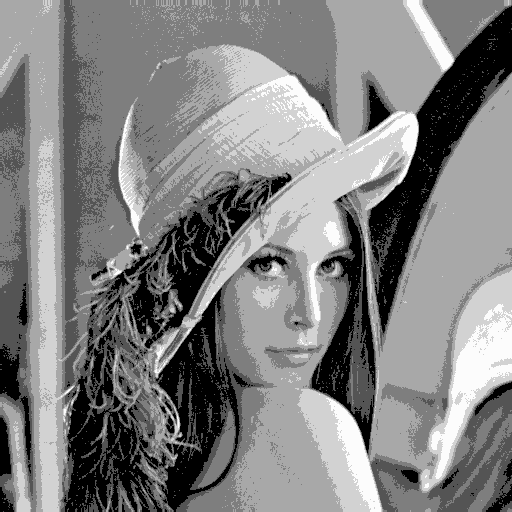
\includegraphics[scale=0.32]{DiminuirBits.png}
\caption{Linearização em $n$ etapas}
\label{fig:rota}
\end{minipage}
\end{figure}
\FloatBarrier
\begin{figure}[!htb]
\begin{minipage}[b]{0.45\linewidth}
\centering
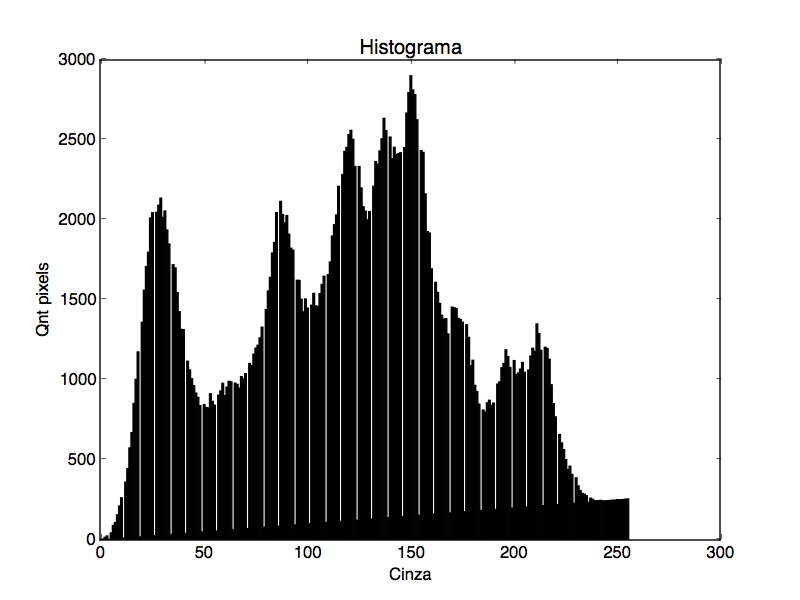
\includegraphics[scale=0.25]{Histo_lena_B.jpg}
\caption{Imagem Original}
\label{fig:original}
\end{minipage}
\hspace{0.5cm}
\begin{minipage}[b]{0.45\linewidth}
\centering
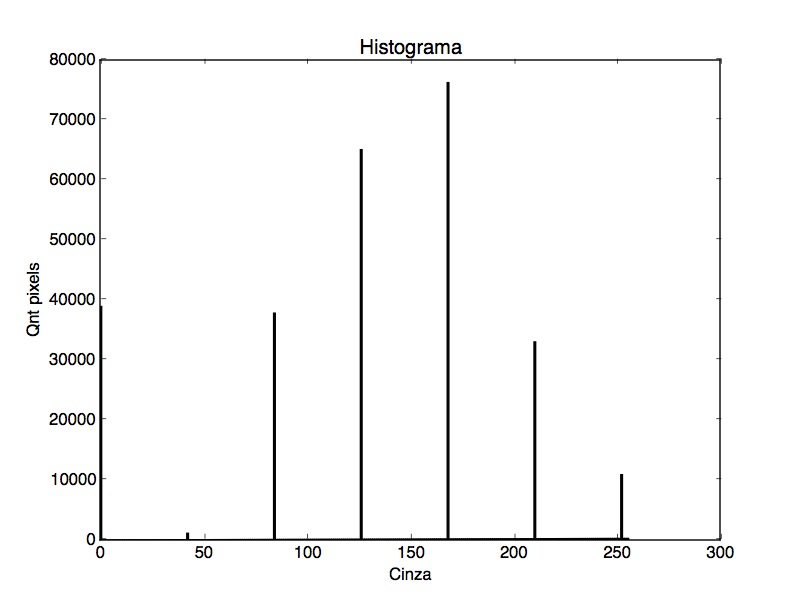
\includegraphics[scale=0.25]{Histo_DiminuirBits.jpg}
\caption{Linearização em $n$ etapas}
\label{fig:rota}
\end{minipage}
\end{figure}
\FloatBarrier

\section{Conclusão}
Concluímos que com funções lineares, não lineares e equalizações, conseguimos ajustar pequenos detalhes nas imagens. A aplicação de contraste e normalização da imagem realça informações visuais antes não visíveis.

Além da questão de qualidade podem ser aplicadas distorções, rotações, translações, escalas (e outras diversas funções) podem ser aplicadas com pequenas funções lineares e não lineares para manipular a matriz de pixeis a favor de obter algum resultado esperado, além de ter o poder de mudar totalmente uma imagem.

\end{document}
